% Chapter II:
\section{Planteamiento del Problema}

\subsection{Situación Problemática}

\Textcite{vonDavier2011} said this, that
too \parencite{vonDavier2011,Lassen2006}.  Further evidence comes from
other sources \parencite{Shotton1989,Lassen2006}.  

\lipsum[3]

\lipsum[4]

\subsection{Formulación del Problema}

\lipsum[4]

\lipsum[5]

\begin{figure}[ht]
  \caption{Cuadro y gráficos que muestran el método N2. Adaptado de \cite{deWaal2009}}
  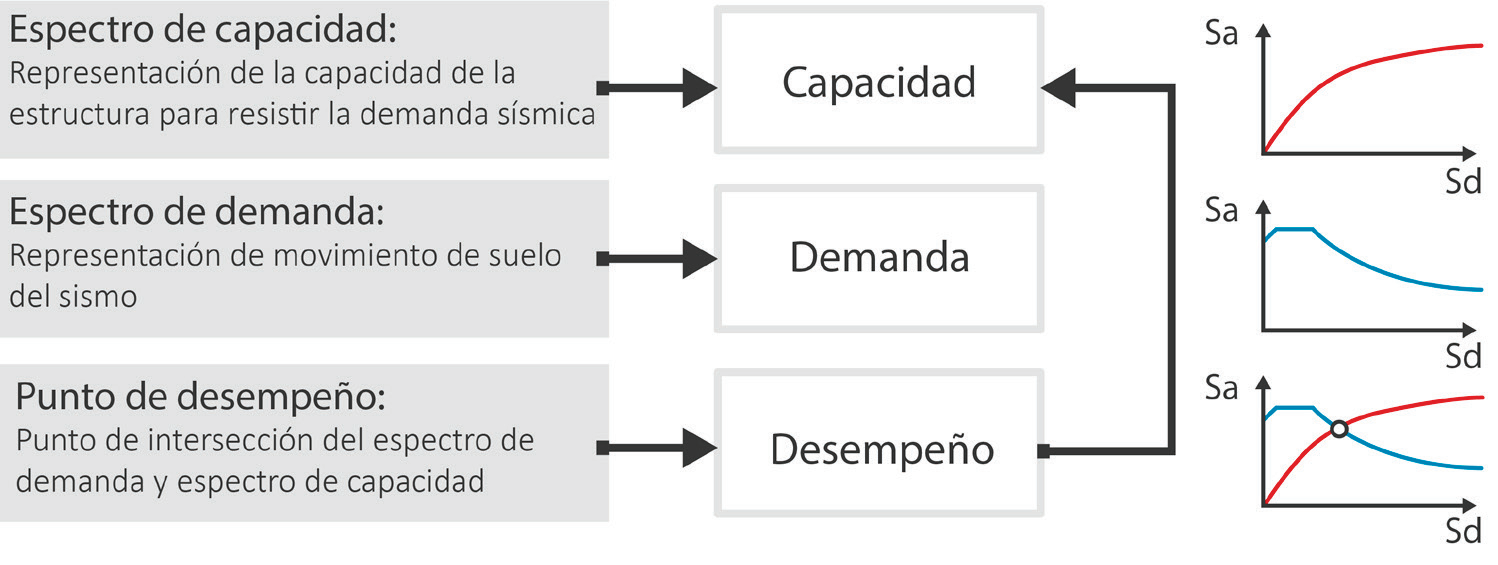
\includegraphics[scale=0.36]{E_IMAGENES/3_Capitulo3/Cap3_Imagen70.png}
  \figurenote{This is a great figure.}
	\label{Cap3_Figura8}
\end{figure}

\subsection{Justificación de la Investigación}

\lipsum[6]

\subsection{Objetivos de la Investigación}

\lipsum[7]

\subsubsection{Objetivo General}

\lipsum[8]

\subsubsection{Objetivos Específicos}

\lipsum[9]

\begin{figure}
  \caption{Figura con subfiguras}
  \label{fig:figura}
  \begin{subfigure}{0.4\textwidth}
      \centering
      \caption{A}
      
\includegraphics[width=\linewidth]{E_IMAGENES/0_Caratula/USIL LOGO.png}
      \label{fig:subfig1}
  \end{subfigure}
  \hfill
  \begin{subfigure}{0.4\textwidth}
      \centering
      \caption{B}
      
\includegraphics[width=\linewidth]{E_IMAGENES/0_Caratula/USIL LOGO.png}
      \label{fig:subfig2}
  \end{subfigure}
  \figurenote{Buenas figuras}
\end{figure}

\subparagraph{Inter-rater reliability}
\lipsum[10]

\subparagraph{Test-retest reliability}
\lipsum[11]

\paragraph{Validity}
\lipsum[12]

\subparagraph{Face validity}
\lipsum[13]

\subparagraph{Construct validity}
\lipsum[14]